% ------------------------------------------------------------------------
% bjourdoc.tex for birkjour.cls*******************************************
% ------------------------------------------------------------------------
%%%%%%%%%%%%%%%%%%%%%%%%%%%%%%%%%%%%%%%%%%%%%%%%%%%%%%%%%%%%%%%%%%%%%%%%%%

\documentclass{birkjour}
%
%
% THEOREM Environments (Examples)-----------------------------------------
%
 \newtheorem{thm}{Theorem}[section]
% \newtheorem{cor}[thm]{Corollary}
% \newtheorem{lem}[thm]{Lemma}
% \newtheorem{prop}[thm]{Proposition}
% \theoremstyle{definition}
 \newtheorem{defn}[thm]{Definition}
% \theoremstyle{remark}
% \newtheorem{rem}[thm]{Remark}
% \newtheorem*{ex}{Example}
 \numberwithin{equation}{section}

\usepackage[noadjust]{cite}
\usepackage{amsfonts}
\usepackage{listings}
\usepackage{algorithm}
\usepackage{algorithmic}
\usepackage{booktabs}
\usepackage{float}
\usepackage{caption}

\begin{document}

%-------------------------------------------------------------------------
% editorial commands: to be inserted by the editorial office
%
%\firstpage{1} \volume{228} \Copyrightyear{2004} \DOI{003-0001}
%
%
%\seriesextra{Just an add-on}
%\seriesextraline{This is the Concrete Title of this Book\br H.E. R and S.T.C. W, Eds.}
%
% for journals:
%
%\firstpage{1}
%\issuenumber{1}
%\Volumeandyear{1 (2004)}
%\Copyrightyear{2004}
%\DOI{003-xxxx-y}
%\Signet
%\commby{inhouse}
%\submitted{March 14, 2003}
%\received{March 16, 2000}
%\revised{June 1, 2000}
%\accepted{July 22, 2000}
%
%
%
%---------------------------------------------------------------------------
%Insert here the title, affiliations and abstract:
%


\title[Robust Quaternion Estimation with Geometric Algebra]
 {Robust Quaternion Estimation with \\Geometric Algebra}

%----------Author 1
\author[Mauricio Cele Lopez Belon]{Mauricio Cele Lopez Belon}
\address{Madrid, Spain}
\email{mclopez@outlook.com}

%----------classification, keywords, date
\subjclass{Parallel algorithms 68W10; Clifford algebras, spinors 15A66}

\keywords{Geometric Algebra, Quaternion Estimation, Wahba Problem}

\date{October 21, 2019}
%----------additions
%\dedicatory{To my wife}
%%% ----------------------------------------------------------------------

\begin{abstract}

Robust methods for finding the best rotation aligning two sets of corresponding vectors are formulated in the linear algebra framework, using tools like the SVD for polar decomposition or QR for finding eigenvectors. Those are well established numerical algorithms which on the other hand are iterative and computationally expensive. Recently, closed form solutions has been proposed in the quaternion's framework, those methods are fast but they have singularities i.e., they completely fail on certain input data. In this paper we propose a robust attitude estimator based on a formulation of the problem in Geometric Algebra. We find the optimal eigen-quaternion in closed form with high accuracy and with competitive performance respect to the fastest methods reported in literature.

\end{abstract}

%%% ----------------------------------------------------------------------
\maketitle
%%% ----------------------------------------------------------------------
%\tableofcontents
\section{Introduction}

\indent The estimation of rotations has been studied for over half a century \cite{Wahba1965}. The problem consist on finding the optimal rotation aligning two sets of corresponding vectors. Many effective methods have been developed \cite{Arun1987, Horn1987, Mortari1996, Shuster1981, Yang2015} using $3\times3$ matrices and quaternions. Formulations based on quaternions solves a max-eigenvalue problem, while formulations based on linear algebra relies on Singular Value Decomposition (SVD). In the last decade formulations based on geometric algebra \cite{Perwass2009, Dorst2011} were introduced but they also rely on linear algebra numerical algorithms such as SVD due to the lack of native numerical algorithms. Closed form solutions for finding the optimal quaternion has been proposed \cite{Yang2013, Wu2017, Wu2018FA3R, Wu2018FS3R} based on analytic formulas for solving the roots of the quartic polynomial associated with eigenvalue problem.

Accuracy and speed of prominent methods have been compared in  \cite{Eggert1997, Markley1999, Wu2017} evidencing a trade-off between performance and robustness. In particular SVD based methods exhibit the best accuracy but low performance and quaternion based methods are faster but less accurate. Regarding the later methods, the closed form solutions exhibit the best performance so far but they have singularities i.e., they completely fail on certain input data.

In this paper we propose a robust estimator of the best quaternion aligning two sets of corresponding vectors. We maximize a convex quadratic energy functional formulated in the $\mathbb{G}_{3,0,0}$ geometric algebra which allow us to find an optimal quaternion in a robust way without resorting to linear algebra numerical algorithms. Geometric algebra rotors are isomorphic to quaternions, we find geometric algebra to be a more natural choice for studying this problem since rotations and subspaces of $\mathbb R^3$ are treated in the same manner, facilitating meaningful algebraic manipulations. We primarily work with bivectos instead of vectors for the sake of mathematical convenience. Due to mathematical (and geometric) duality of vectors and bivectors in $\mathbb{G}_3$ our formulation is also valid for vectors.

\section{Geometric Algebra $\mathbb{G}_3$}

A geometric algebra $\mathbb{G}_3$ is constructed over a real vector space $\mathbb R^3$, with basis vectors $\{e_1, e_2, e_3\}$. The associative geometric product is defined on vectors so that the square of any vector $a$ is a scalar $a a = a^2 \in \mathbb{R}$ and the geometric product of two vectors $a$ and $b$ is $a b = a \cdot b + a \wedge b$ and $b a = b \cdot a - a \wedge b$. From the vector space $\mathbb R^3$, the geometric product generates the geometric algebra $\mathbb{G}_3$ with elements $\{ X, R, A...\}$ called multivectors.

For a pair of vectors $a$ and $b$, a symmetric inner product $a \cdot b = b \cdot a$ and antisymmetric outer product $a \wedge b = -b \wedge a$ can be defined implicitly by the geometric product. It is easy to prove that $a \cdot b = \frac{1}{2}(a b + b a)$ is a scalar, while the quantity $a \wedge b = \frac{1}{2}(a b - b a)$, called a bivector or $2$-vector, is a new algebraic entity that can be visualized as the two-dimensional analogue of a direction i.e., a planar direction. Similar to vectors, bivectors can be decomposed in a bivector basis $\{ e_{12}, e_{13}, e_{23} \}$ where $e_{ij} = e_i \wedge e_j$.

The outer product of three vectors $a \wedge b \wedge c$ generates a $3$-vector also known as the pseudoscalar, because the trivector basis consist of single element $e_{123} = e_1 \wedge e_2 \wedge e_3$. Similarly, the scalars are regarded as $0$-vectors whose basis is the number $1$. It follows that the outer product of $k$-vectors is the completely antisymmetric part of their geometric product: $a_1 \wedge a_2 \wedge ... \wedge a_k = \langle a_1 a_2 ... a_k \rangle_k$ where the angle bracket means $k$-vector part, and $k$ is its grade. The term grade is used to refer to the number of vectors in any exterior product. This product vanishes if and only if the vectors are linearly dependent. Consequently, the maximal grade for nonzero $k$-vectors is $3$. It follows that every multivector $X$ can be expanded into its $k$-vector parts and the entire algebra can be decomposed into $k$-vector subspaces:
\begin{equation*}
\mathbb G_3 = \sum_{k=0}^n{\mathbb{G}^k_3} = \{ X = \sum_{k=0}^n { \langle X \rangle_k } \}
\end{equation*}
This is called a \emph{grading} of the algebra. 

Reversing the order of multiplication is called reversion, as expressed by $(a_1 a_2 ... a_k)\tilde{} = a_k ... a_2 a_1$ and $(a_1 \wedge a_2 \wedge ... \wedge a_k)\tilde{} = a_k \wedge ... \wedge a_2 \wedge a_1$, and the reverse of an arbitrary multivector is defined by $\tilde{X} = \sum_{k=0}^n { \langle \tilde{X} \rangle_k }$.

\subsection{Rotors}

Rotations are even grade multivectors known as rotors. We denote the subalgebra of rotors as $\mathbb{G}^{+}_3$. A rotor $R$ can be generated as the geometric product of an even number of vectors. A reflection of any $k$-vector $X$ in a plane with normal $n$ is expressed as the sandwitch product $(-1)^k n X n$. The most basic rotor $R$ is defined as the product of two unit vectors $a$ and $b$ with angle of $\frac{\theta}{2}$. The rotation plane is the bivector $L = \frac{a \wedge b}{\| a \wedge b \|}$.
\begin{equation}
a b = a \cdot b + a \wedge b = \cos\left( \frac{\theta}{2} \right) + L \sin\left( \frac{\theta}{2} \right).
\end{equation}
Rotors act on all $k$-vectors using the sandwitch product $X' = R X \tilde R$, where $\tilde R$ is the reverse of $R$ and can be obtained by reversing the order of all the products of vectors.

\subsection{Bivector products}

We define the commutator product of two bivectors $p_j$ and $q_j$ as $p_j \times q_j = \frac{1}{2}(p_j q_j - q_j p _j)$. The commutator product of bivectors in $\mathbb{G}_3$  can be interpreted as a cross-product of bivectors i.e., the resulting bivector $B = p_j \times q_j$ is orthogonal to both $p_j$ and $q_j$. The commutator product allow us to define the geometric product of two bivectors as $A B = A \cdot B + A \times B$. The inner product of bivectors differs from the inner product of vectors on the sign, since the square of bivectors is negative, the inner product of bivectors is a negative scalar e.g., $(a e_{12} + b e_{13} + c e_{23}) \cdot (d e_{12} + e e_{13} + f e_{23}) = -a d - b e - c f$.

\subsection{Quaternions}

A quaternion $Q = w + \vec v$ consists of two parts: a scalar part $w$ and vector part $\vec v$ which denotes the axis of rotation. The vector part $\vec v$ is defined in a basis of complex vectors $\{ i, j, k \}$ that squares to $-1$ and anticommute i.e., $i^2 = j^2 = k^2 = -1$ and $i j k = -1$. In geometric algebra they corresponds to bivectors:
\begin{eqnarray}
i = e_{23} \ \ \ j = e_{13} \ \ \  k = e_{12} \\
ijk = e_{23} e_{13} e_{12} = -1 \nonumber
\end{eqnarray}
Rotors can easily be transformed to quaternions and vice versa. A rotor $R = w + L$ corresponds with a quaternion $Q = w + \vec v$, where $L = \alpha e_{12} + \beta e_{13} + \gamma e_{23}$ and $\vec v = \gamma i + \beta j + \alpha k$.

\section{Geometric Algebra Rotor Estimation}

Given two sets of $n$ corresponding bivectors $P = \{p_j\}_{j=1}^n$ and $Q = \{q_j\}_{j=1}^n$, we attempt to maximize the following energy function:
\begin{eqnarray}
	E(R) = \max_{R \in \mathbb{G}^{+}_3 } \sum_j { c_{j} \|p_j + \tilde R q_i R \|^2 }\\
	s.t. \ R \tilde R = 1 \nonumber
\end{eqnarray}
where $\{c_{j}\}_{j=1}^n$ are scalar weights such that $\sum_j^n{c_j} = 1$. It is a quadratic maximization problem with a non-linear constraint in $R$. Notice that the term $\|p_j + \tilde R q_i R\|^2$ is dual to the traditional least squares error $\|q_j - R p_j \tilde R\|^2$. Duality in the sense that the optimal $R$ is a critical point of both energies.
Notice also that $p_j + \tilde R q_i R$ is equivalent to $R p_j + q_j R$ by multiplying by $R$ on the left and using the fact that $R \tilde R = 1$. The equivalent problem is:
\begin{eqnarray}
	\label{eqn:max_energy}
	E(R) = \max_{R \in \mathbb{G}^{+}_3 } \sum_j { c_{j} \|R p_j + q_j R\|^2 }\\
	s.t. \ R \tilde R = 1 \nonumber
\end{eqnarray}
which exposes the that $R$ is only quadratic in \ref{eqn:max_energy}.

The constraint $R p_j + q_j R$ can be rewriten as $(w + L) p_j  + q_j (w + L)$. For some a scalar $w$ and bivector $L$. Expanding the geometric product of bivectors in terms of the inner product and the communtator product we get:
\begin{eqnarray}
	w  (p_j + q_j) + L \cdot (p_j + q_j)  + (q_j - p_j) \times L
\end{eqnarray}

In matrix language we can define the following matrix system $M_j R = 0$:
\begin{eqnarray}
	M_j R =
	\left[\begin{array}{cc}
		0      &       -s_j^T \\
		s_j    &   \left[ d_j \right]_\times \\
	\end{array}\right]
	\left[\begin{array}{c} 
		w \\
		L
	\end{array}\right] = 
	\left[\begin{array}{c}
		-s_j^T L \\
		w s_j + d_j \times L 
	\end{array}\right]\\
	d_j = q_j - p_j \ \ s_j = p_j + q_j  \nonumber
\end{eqnarray}
where $d_j$ and $s_j$ are $3 \times 1$ column vectors holding bivector's coefficients, $M_j$ is a skew-symmetric $4\times 4$ real matrix, so that $M_j^T = -M_j$. The rotor $R$ is represented as $4 \times 1$ column vector made of the scalar $w$ and the $3 \times 1$ column vector $L$ holding the bivector's components. The $3\times 3$ matrix $\left[ d_j \right]_\times$ is representing the skew-symmetric cross-product matrix as usually defined for vectors in $\mathbb R^3$.

We can express $E(R)$ as the following quadratic form:
\begin{eqnarray}
E(R) = \max_R R^T M R\\
s.t. \ R^T R = 1  \nonumber
\end{eqnarray}
where $M = \sum_j^n { c_j M_j^T M_j}$. Note that since $M_j$ is skew-symmetric, the product $M_j^T M_j$ is symmetric and positive semi-definite.
Consequently the matrix $M$ is also symmetric positive semi-definite. It follows that all eigenvalues of $M$ are real and $\lambda_i \geq 0$.
\begin{eqnarray}
	M_j^T M_j = 
	\left[\begin{array}{cc}
		\| s_j \|^2       &         (s_j \times d_j)^T \\
		s_j \times d_j  &    s_j s_j^T - \left[ d_j \right]^2_\times \\
	\end{array}\right]\\
	d_j = q_j - p_j \ \ s_j = p_j + q_j  \nonumber
\end{eqnarray}

By the spectral theorem the maximizer of $E(R)$ is the eigenvector of $M$ associated with the largest eigenvalue which is a positive number.

\section{Convexity}

The convexity of the energy $E(R)$ can be proof by showing that its Hessian matrix of second partial derivatives is positive semi-definite. The Hessian matrix of $E(R)$ is $\frac{\partial^2 E(R)}{\partial R} = \sum_j^n { c_j M_j^T M_j}$ which is symmetric, moreover since $M_j$ is skew-symmetric matrix, the product $M_j^T M_j$ is symmetric positive semi-definite. Then follows that $\sum_j^n { c_j M_j^T M_j}$ is positive semi-definite and therefore convex, provided that the sum of weights is convex i.e., $\sum_j^n { c_j } = 1$.

\section{Optimal Quaternion using 4D Geometric Algebra}

The most time consuming task of the estimation is to compute the eigenvector of $M$ associated with the greatest eigenvalue. In this section we show how to find the largest eigenvalue and its corresponding eigenvector i.e., the required quaternion, using the 4D Geometric Algebra $ \mathbb{G}_4$ which is robust, efficient and accurate.

Let us define four vectors $\textbf m_1$, $\textbf m_2$, $\textbf m_3$, $\textbf m_4$ corresponding to the columns of matrix $M$:
\begin{eqnarray}
	M = \sum_j^n { c_j M_j^T M_j} =
	\left[\begin{array}{cccc}
		\\
		\textbf m_1 & \textbf m_2 & \textbf m_3 & \textbf m_4 \\
		\\
	\end{array}\right]
\end{eqnarray}

The matrix system that we want to solve is $M R = \lambda R$ for $\lambda$ corresponding to the largest eigenvalue of $M$. We can write the system in its homogeneous form:
\begin{eqnarray}
	\label{eqn:eigensystem}
	\left[\begin{array}{cccc}
		\\
		\textbf m_1 - \lambda e_1 & \textbf m_2 - \lambda e_2 & \textbf m_3 - \lambda e_3 & \textbf m_4- \lambda e_4 \\
		\\
		\\
	\end{array}\right]
	\left[\begin{array}{c} 
		w \\
		L_1\\
		L_2\\
		L_3
	\end{array}\right] = 	
	\left[\begin{array}{c} 
		0 \\
		0 \\
		0 \\
		0
	\end{array}\right]
\end{eqnarray}

The matrix in equation~\ref{eqn:eigensystem}, called \emph{characteristic matrix}, is of rank $3$ and thus singular i.e., the vectors $(\textbf m_1 - \lambda e_1)$, $(\textbf m_2 - \lambda e_2)$, $(\textbf m_3 - \lambda e_3)$ and $()\textbf m_4- \lambda e_4)$ are linearly dependent. It follows that its outer product must be zero:
\begin{eqnarray}
\label{eqn:characteristic_outer_product}
(\textbf m_1 - \lambda e_1)\wedge(\textbf m_2 - \lambda e_2)\wedge(\textbf m_3 - \lambda e_3)\wedge(\textbf m_4- \lambda e_4) = 0
\end{eqnarray}

Which is called the \emph{charactetistic outer porduct} and is equivalent to the characteristic polynomial $P(\lambda) = det(M - \lambda I)$. A simple way to find the largest eigenvalue is using Newton-Raphson method $\lambda_{i+1} = \lambda_i - P(\lambda) / P'(\lambda)$. This method is indeed robust given that all eigenvalues are non-negative real numbers, it wasn't however for methods based on Davenport's matrix \cite{Davenport1968} which eigenvalues can be negative. We found that $Trace(M)$ is a robust guess for Newton-Raphson iteration because it is larger than the largest eigenvalue and is also close enough to converge in few iterations. For the sake of completeness we show the first derivative of \ref{eqn:characteristic_outer_product}:
\begin{eqnarray*}
P'(\lambda) = 
- e_1\wedge(\textbf m_2 - \lambda e_2)\wedge(\textbf m_3 - \lambda e_3)\wedge(\textbf m_4- \lambda e_4)\\
- (\textbf m_1 - \lambda e_1)\wedge e_2\wedge(\textbf m_3 - \lambda e_3)\wedge(\textbf m_4- \lambda e_4)\\
- (\textbf m_1 - \lambda e_1)\wedge(\textbf m_2 - \lambda e_2)\wedge e_3\wedge(\textbf m_4- \lambda e_4)\\
- (\textbf m_1 - \lambda e_1)\wedge(\textbf m_2 - \lambda e_2)\wedge(\textbf m_3 - \lambda e_3)\wedge e_4
\end{eqnarray*}

Following \cite{DeKeninck2019} we solve the system~\ref{eqn:eigensystem} using outer products. For a linear system $A \textbf x = b$ the authors in \cite{DeKeninck2019} defines $N$ linear equations of the form $A^T_j \textbf x = b_j$ each of which corresponds to a dual hyper-plane of the form $\textbf a_j \equiv A_j - b_j e_0$ where the solution $\textbf x$ must lie on. The $e_0$ is an \emph{homogeneous} basis vector needed for enabling projective geometry, enlarging the base space to $N+1$, which interpretation is to be the offset of the hyper-plane. So solution of the linear system is the intersection of $N$ dual hyper-planes, which is given by its outer product.
\begin{eqnarray}
\alpha (\textbf x + e_0)^* = \textbf a_1 \wedge \textbf a_2 \wedge ... \wedge \textbf a_N
\end{eqnarray}

Where the symbol $^*$ is the dual operator of the $N+1$ space and $\alpha$ is a weight factor. After taking the dual of $\alpha (\textbf x + e_0)^*$ and divide by the coefficient of $e_0$ (which is $\alpha$), the solution $\textbf x$ can be read off the coefficients of the $1$-vector.

We know that the null space of $(M - \lambda I)$ is of rank one. Algebraically this means that one of its column vectors is redundant i.e., it can be written in term of the others. In linear algebra this means that the system has infinitely many solutions. The geometric interpretation is that all hyper-planes intersect in a line passing through the origin. Since all solutions lie on the same line and they only differ by a scaling term, a particular solution can be found by fixing the scale. Actually, it is enough to constrain the scale of a single hyper-plane. The homogeneous component $e_0$ can be interpreted as scale of solution (instead of hyper-plane's offset as in \cite{DeKeninck2019}) since it affects only that aspect of the solution. In linear algebra language it is equivalent to set one value at the right hand side of \ref{eqn:eigensystem}, however that system can't be solved in linear algebra because it requires to invert a singular matrix.

We define the dual hyper-planes passing through the origin as:
\begin{eqnarray}
   \textbf a_i \equiv \textbf m_i - \lambda e_i
\end{eqnarray}

Although in most cases it is enough to set the scale of a single hyper-plane go get a solution it is inconvenient to do so, as will be explained in Section~\ref{section:robustness}. It is more robust to set the scale of all hyper-planes to some $\gamma \neq 0$ which is a scalar value. Intersection can then be found by taking the outer product as:
\begin{eqnarray}
\label{eqn:hyperplanes_intersection}
\alpha (\textbf x + 1)^* = (\textbf a_1 + \gamma) \wedge  (\textbf a_2 + \gamma) \wedge  (\textbf a_3  + \gamma) \wedge (\textbf a_4 + \gamma)
\end{eqnarray}

Distributing the outer product and keeping the terms of grade-$3$ we get:
\begin{eqnarray}
\alpha (\textbf x + 1)^* =  \gamma (\textbf a_1 \wedge \textbf a_3 \wedge \textbf a_4
+ \textbf a_1 \wedge \textbf a_2 \wedge \textbf a_4
+ \textbf a_1 \wedge \textbf a_2 \wedge \textbf a_3
+ \textbf a_2 \wedge \textbf a_3 \wedge \textbf a_4)
\end{eqnarray}

Here the symbol $^*$ is the dual operator of the $4$D space (not $5$D as in \cite{DeKeninck2019} which allow us to be more efficient) and $\alpha$ is a weight factor. After taking the dual of $\alpha (\textbf x + 1)^*$ the eigenvector $\textbf x$ can be read off the coefficients of the $1$-vector. Notice that solution needs to be normalized.

\section{Optimal Computation of M}

The symmetric matrix $M_j^T M_j$ has a simple form:

\begin{eqnarray*}
	M_j^T M_j = 
	\left[\begin{array}{cc}
		\| s_j \|^2        &         (s_j \times d_j)^T \\
		s_j \times d_j  &    s_j s_j^T - d_j d_j^T + \| d_j \|^2 I \\
	\end{array}\right]\\
	d_j = q_j - p_j \ \ s_j = p_j + q_j
\end{eqnarray*}

Writing it in terms of $p_j$ and $q_j$ we get:

\begin{eqnarray}
   \label{eqn:matrix_fast}
   	M_j^T M_j = 2
	\left[\begin{array}{cc}
		p_j^T q_j       &         (p_j \times q_j)^T \\
		p_j \times q_j  &    p_j q_j^T + q_j p_j^T - p_j^Tq_j I_{3\times3} \\
	\end{array}\right]
    + (\| p_j \|^2 + \| q_j \|^2) I_{4\times4}
\end{eqnarray}
All terms of \ref{eqn:matrix_fast} can be derived from the covariance matrix $B = p_j q_j^T$ plus the quantity $\| p_j \|^2 + \| q_j \|^2$. Since matrix $B$ is of $3\times3$ its computation is more efficient than the whole \ref{eqn:matrix_fast}. Details can be found in Section~\ref{section:algoritms}.

\section{Robustness and Singularities}
\label{section:robustness}

As stated before, setting the scale of a single hyperplane is enough to get a valid eigenvector in most cases. However, the choice of which hyper-plane to constraint is problematic. For instance,  assuming input vectors without noise, constraining the hyperplane corresponding to the $w$ component of the rotor won't work because when the angle of rotation is $\pi$ the $w = \cos(\pi/2) = 0$ and so its scale cannot be constrained. Similarly, constraining one of the hyper-planes corresponding to $L_1$, $L_2$ or $L_3$ won't work because when the angle of rotation is $0$ or $4 \pi$ the $\sin(2 \pi) = 0$ and so on. Then, it is complex task to avoid all problematic situations. By constraining all hyper-planes as in \ref{eqn:hyperplanes_intersection} our geometric algebra method does not suffer from any of those singularities.

Some of the above mentioned singularities are present in classic methods such as QUEST \cite{Shuster1981} and FOMA \cite{Markley1993} but also on methods derived from those, including recent descendants based on analytic formulas \cite{Yang2013, Wu2016, Wu2017, Wu2018FA3R, Wu2018FS3R}. All those methods are based on finding the eigenvector corresponding to largest eigenvalue of Davenport's matrix \cite{Davenport1968}. Since that is an indefinite matrix, some eigenvalues are positive and some negative, the Newton-Raphson can fail to find the max eigenvalue (which can be negative). So significant effort has been put on finding fast and robust analytic solutions to the quartic polynomial but no advances has been made on improving robustness on finding the associated eigen-vector besides doing \emph{sequential rotations} i.e., a $\pi$ angle rotation of input data accomplished by changing the signs of two columns of the covariance matrix of \cite{Shuster1981}. The QUEST method performs sequential rotations one axis at a time, until an acceptable reference coordinate system is found.

\section{Algorithms}
\label{section:algoritms}

The pseudo-code of proposed method is shown in Algorithm~\ref{alg:FastRotorEstimation}. 

\begin{algorithm}
\begin{algorithmic}[1]
\REQUIRE {$P = \{p_{j}\}_{j=1}^n, Q = \{q_{j}\}_{j=1}^n, C = \{c_{j}\}_{j=1}^n$}
\STATE{$S = B = 0, \gamma = 1$}
\FOR{$j = 1$ \TO $n$}
\STATE{$S = S + c_j (p_j \cdot p_j + q_j \cdot q_j)$}
\STATE{$B = B + c_j p_j q_j^T$}
\ENDFOR
\STATE{$\textbf m_1 = (\frac{1}{2}S + Tr(B)) e_1 + (B_{12} - B_{21}) e_2 + (B_{20} - B_{02}) e_3 + (B_{01} - B_{10}) e_4$}
\STATE{$\textbf m_2 = (B_{12} - B_{21})e_1 + (2 B_{00} + \frac{1}{2}S - Tr(B)) e_2 + (B_{01} + B_{10}) e_3 + (B_{20} + B_{02}) e_4$}
\STATE{$\textbf m_3 = (B_{20} - B_{02})e_1 + (B_{01} + B_{10}) e_2 + (2 B_{11} + \frac{1}{2}S - Tr(B)) e_3 + (B_{12} + B_{21}) e_4$}
\STATE{$\textbf m_3 = (B_{01} - B_{10})e_1 + (B_{20} + B_{02} ) e_2 + (B_{12} + B_{21}) e_3 + (2 B_{22} + \frac{1}{2}S - Tr(B)) e_4$}
\COMMENT{Newton-Raphson}
\STATE{$\lambda_0 = 7 S - 3 Tr(B)$}
\REPEAT
\STATE{$\lambda_{i+1} = \lambda_i - P(\lambda_i) / P'(\lambda_i)$}
\UNTIL{$\|\lambda_{i+1} - \lambda_i\| < \epsilon$}
\STATE{$\textbf a_1 = \textbf m_1 - \lambda e_1$
}
\STATE{$\textbf a_2 = \textbf m_2 - \lambda e_2$
}
\STATE{$\textbf a_3 = \textbf m_3 - \lambda e_3$
}
\STATE{$\textbf a_4 = \textbf m_4 - \lambda e_4$
}
\STATE{$\textbf X = \gamma (\textbf a_1 \wedge \textbf a_3 \wedge \textbf a_4
	+ \textbf a_1 \wedge \textbf a_2 \wedge \textbf a_4
	+ \textbf a_1 \wedge \textbf a_2 \wedge \textbf a_3
	+ \textbf a_2 \wedge \textbf a_3 \wedge \textbf a_4)$}
\STATE{$R = normalize( \langle \textbf X^* \rangle_1 )$}
\RETURN { $R(0) + R(1) e_{12} + R(2) e_{13} + R(3) e_{23}$ }
\end{algorithmic}
\caption{Fast Rotor Estimation}\label{alg:FastRotorEstimation}
\end{algorithm}
An optimized C++ code using the Eigen library \cite{Eigen} and GAALOP  \cite{Gaalop} is publicly available on GitHub \cite{GARotorEstimator}

\section{Comparisons}

We selected several representative methods e.g. FLAE \cite{Wu2017}, SVD \cite{Arun1987}, QUEST \cite{Shuster1981}, FA3R \cite{Wu2018FA3R}, Symbolic \cite{Wu2018FS3R}, Q-Method \cite{Shuster1981} and FOMA \cite{Markley1993} for comparison. The Eigen library \cite{Eigen} was employed to implement all of them. The tests were ran on a MacBook Pro laptop with Intel Core i7 CPU running at 2,5 GHz. The Clang C++ compiler was used with -Ofast option enabled.

We first show that some methods fails on producing meaningful rotations when certain input data is provided. Table~\ref{tab:failure_cases} shows four cases which causes error. First two cases consist of having input vectors rotated $\pi/2$ and $\pi$ radians without noise. Other case is when the 3D vectors are projected to the $YZ$-plane and rotated  around the $X$-axis without noise. The last case is similar but projected to the $XZ$-plane. The root mean-squared error (RMSE) is used to describe the difference of accuracy.

 \begin{table} [H]
 \centering
 \resizebox{1.0\textwidth}{!}{ 
 \begin{tabular}{cccccc}
 \toprule
 {Algo}&{$\pi/2$}&{$\pi$}&{$YZ$Plane}&{$XZ$Plane}&{$XY$Plane}\\
 \midrule
 {FLAE}&{$4.41 \times 10^{-28}$}&{$696$}&{$392$}&{$1328$}&{$3.25 \times 10^{-28}$}\\
 {Symbolic}&{$1.78 \times 10^{-26}$}&{$1053$}&{$392$}&{$1321$}&{$4.70 \times 10^{-27}$}\\
 {FA3R}&{$4.00 \times 10^{-28}$}&{$5.41 \times 10^{-29}$}&{$2.25 \times 10^{-09}$}&{$2.76 \times 10^{-08}$}&{$4.98 \times 10^{-08}$}\\
 {Proposed}&{$7.32 \times 10^{-18}$}&{$1.79 \times 10^{-18}$}&{$4.05 \times 10^{-28}$}&{$3.43 \times 10^{-28}$}&{$2.22 \times 10^{-24}$}\\
 {Q-Method}&{$3.78 \times 10^{-28}$}&{$2.89 \times 10^{-29}$}&{$7.10 \times 10^{-28}$}&{$1.45 \times 10^{-28}$}&{$9.57 \times 10^{-29}$}\\
 {QUEST}&{$82.6$}&{$2.18 \times 10^{-29}$}&{$6.09 \times 10^{-26}$}&{$9.93 \times 10^{-28}$}&{$8.36 \times 10^{-29}$}\\
 {FOMA}&{$6.08 \times 10^{-28}$}&{$2.95 \times 10^{-28}$}&{$3.93 \times 10^{-26}$}&{$2.13 \times 10^{-27}$}&{$1.19 \times 10^{-28}$}\\
 {SVD}&{$4.41 \times 10^{-28}$}&{$7.51 \times 10^{-29}$}&{$3.35 \times 10^{-28}$}&{$9.83 \times 10^{-29}$}&{$1.09 \times 10^{-28}$}\\
\bottomrule
 \end{tabular}}
 \caption{RMSE of one million vector alignments of a thousand input vectors without noise. Some methods failed when 3D vectors were rotated $\pi/2$ and $\pi$  and when vectors are projected to the coordinate planes}  
 \label{tab:failure_cases}
 \end{table}

We also compared the robustness of the methods when input data has extreme noise applied to the length of input vectors. Figure~\ref{fig:robustness} shows that some methods often fails to find meaningful rotations. We took SVD as reference. Notice that the amount of RMSE is almost the same on successes and on failures, evidencing that almost all methods builds, in essence, the Q-Method's matrix.
 
\begin{figure}[H]
\centering
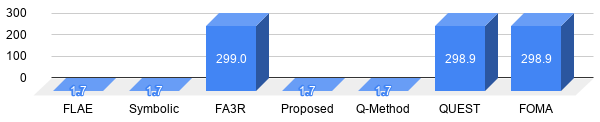
\includegraphics[width=1.0\textwidth]{robustness.png}
\caption{Sum of RMSE of one million vector alignments of a thousand input vectors. We applied Gaussian random noise to angles and random noise to lengths}
\label{fig:robustness}
\end{figure}

Among the compared methods SVD, Q-Method and the ours are the most robust. Performance is shown in Figure~\ref{fig:time} compared to the other methods. Our experiments shows that when the number of input vectors is up to 1000 our method is faster than Q-Method. Beyond that point the trend shows that Q-Method is faster.

\begin{figure}[H]
	\centering
	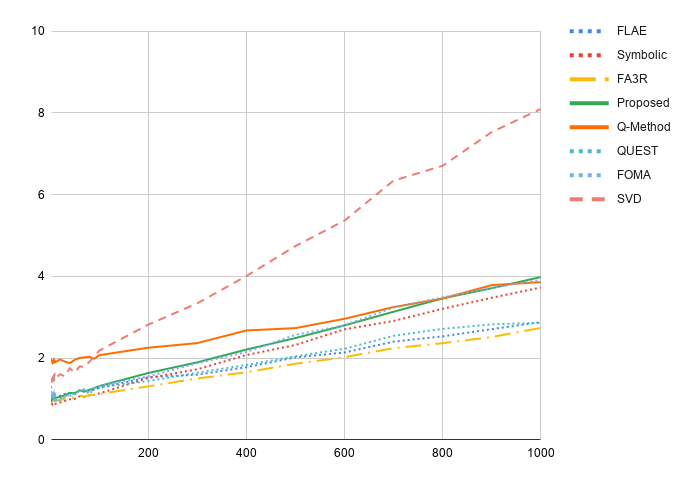
\includegraphics[width=1.0\textwidth]{time.png}
	\caption{Performance comparison: number of vectors v.s. execution time ($\mu$s)}
	\label{fig:time}
\end{figure}

\section{Conclusion}

We presented a novel method for estimating the best quaternion aligning two sets of corresponding vectors and bivectors. Since we maximize a convex energy functional we only deal with non-negative eigenvalues, which makes Newton-Raphson iteration robust. We find the eigenvector corresponding to the largest eigenvalue intersecting hyper-planes in the language of geometric algebra. Results shows that our method is a good alternative in terms of robustness and accuracy. Its speed is competitive when the number of input vectors is relatively small. 


\bibliographystyle{abbrv}
\bibliography{rotorestimation}

% ------------------------------------------------------------------------
\end{document}
% ------------------------------------------------------------------------
